\documentclass[12pt,letterpaper,titlepage,en-US]{article}

\usepackage{basicstyle}
\usepackage{report}
\usepackage{knit}

\definecolor{lbcolor}{rgb}{0.969, 0.969, 0.969} 
\setlength\parindent{0pt}
 \lstset{ 
    language=C++, % choose the language of the code
    basicstyle=\fontfamily{pcr}\selectfont\footnotesize\color{black},
    keywordstyle=\color{black}, % style for keywords
    numbers=none, % where to put the line-numbers
    numberstyle=\tiny, % the size of the fonts that are used for the line-numbers     
    backgroundcolor=\color{lbcolor},
    showspaces=false, % show spaces adding particular underscores
    showstringspaces=false, % underline spaces within strings
    showtabs=false, % show tabs within strings adding particular underscores
    frame=single, % adds a frame around the code
    tabsize=2, % sets default tabsize to 2 spaces
    rulesepcolor=\color{gray},
    rulecolor=\color{black},
    captionpos=b, % sets the caption-position to bottom
    breaklines=true, % sets automatic line breaking
    breakatwhitespace=false, 
}
%
% Homework Details
%   - Title
%   - Due date
%   - Class
%   - Section/Time
%   - Instructor
%   - Author
%

\newcommand{\hmwkTitle}{Mini Project \#6}
\DTMsavetimestamp{DueDate}{2019-05-02T10:00:00-06:00}
\newcommand{\hmwkClass}{CS 6313.001}
\newcommand{\hmwkClassName}{Statistical Methods for Data Science}
\newcommand{\hmwkClassInstructor}{Instructor: Prof.Min Chen}
\newcommand{\hmwkAuthorName}{Shyam Patharla}
\newcommand{\hmwkAuthorNetID}{sxp178231}

\newcommand{\hmwkAuthorOneName}{Lizhong Zhang (lxz160730)}
\newcommand{\hmwkAuthorTwoName}{Hanlin He (hxh160630)}



%
% Title Page
%

\title{
    \vspace{1in}
    \textmd{\textbf{\hmwkClassName \\\hmwkClass:\ \hmwkTitle }}\\
    \normalsize\vspace{0.1in}\small{Due\ on\ \DTMusedate{DueDate}\ at \DTMusetime{DueDate} }\\
    \vspace{0.1in}\large{\textit{\hmwkClassInstructor}}\\
    \vspace{0.5in}
\includegraphics[height=2.4em]{UTD_logo_BW}\\
    \vspace{2in}
}

\author{\textbf{\hmwkAuthorName\ \footnotesize{(\hmwkAuthorNetID)}} \\ }
\date{}
\makeindex

\begin{document}
\maketitle

\pagenumbering{Roman}
\tableofcontents
\pagebreak
\pagenumbering{arabic}


\section{Answers}
First, we constructed the boxplot of the response variable \textbf{psa} as shown below.

\begin{figure}[H]
    \centering
    \caption{Boxplot of the Original PSA Level}\label{obp}
    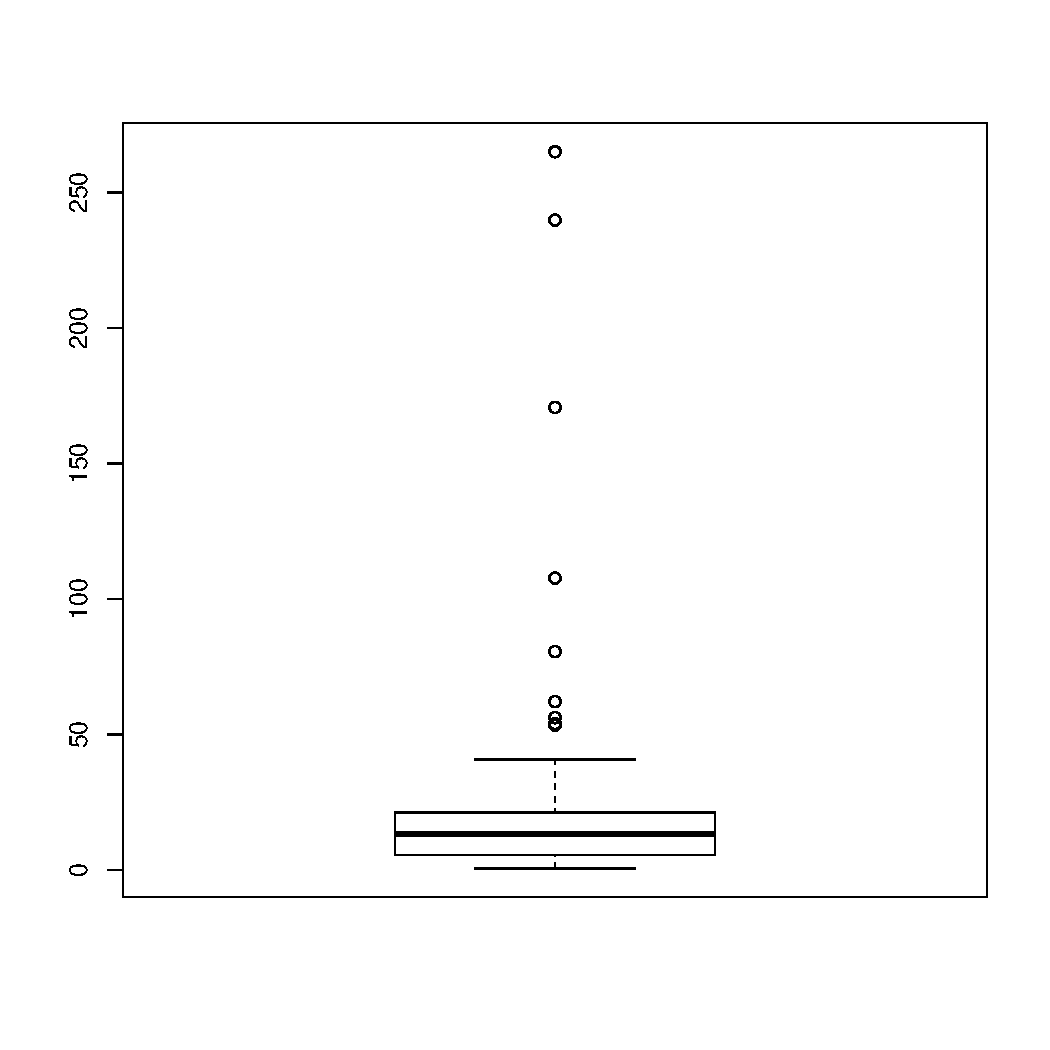
\includegraphics[width=.7\textwidth]{fig/boxplotpsa.pdf}
\end{figure}

Clearly we see many outliers in the boxplot.
To eliminate these outliers, we try transforming the original psa data to
its \textbf{square root} and \textbf{logarithm}, as shown below.

\begin{figure}[H]
    \centering
    \begin{subfigure}[t]{0.5\textwidth}
        \centering
        \caption{Square Root}\label{obptsqrt}
        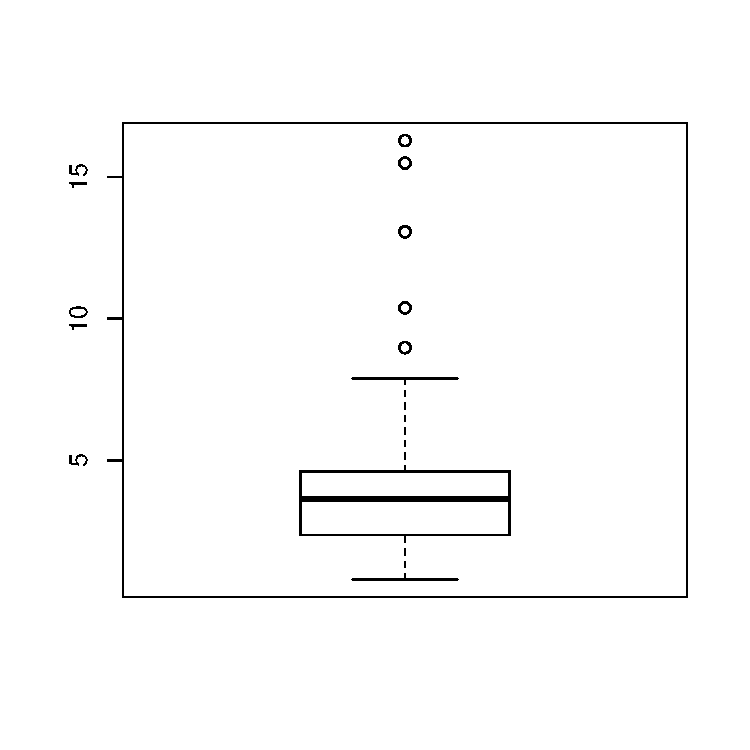
\includegraphics[width=.95\textwidth]{fig/boxplotpsasqrt.pdf}
    \end{subfigure}%
    ~
    \begin{subfigure}[t]{0.5\textwidth}
        \centering
        \caption{Natural Logarithmic Value}\label{obptlog}
        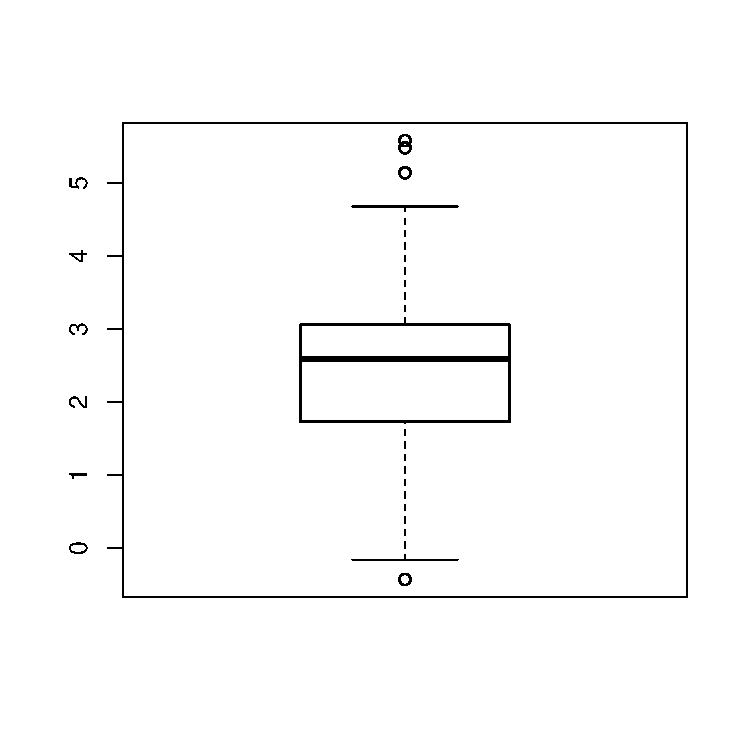
\includegraphics[width=.95\textwidth]{fig/boxplotpsalog.pdf}
    \end{subfigure}
    \caption{Boxplots for square root and logarithm of \textit{psa} variable}\label{obpt}
\end{figure}

We can see that the distribution of natural logarithmic values has less outliers and is closer to a normal distribution than the distribution of the square root of psa. Thus, we continue with our analysis using the natural logarithmic value of the PSA Level.

The following are quantitative predictors:
\begin{enumerate}[leftmargin=*]
    \item Cancer Volume ($cancervol$)
    \item Weight ($weight$)
    \item Age ($age$)
    \item Benign prostatic hyperplasia ($benpros$)
    \item Capsular penetration ($capspen$)
\end{enumerate}


Seminal vesicle invasion ($vesinv$) and Gleason score ($gleason$) are qualitative variables. We first build our model based on quantitative variables.

We now construct scatter plots of log(psa) with each of the quantitative variables, as shown below.

\begin{figure}[H]
    \centering
    \begin{subfigure}[t]{0.5\textwidth}
        \centering
        \caption{Cancer Volume ($cancervol$)}
        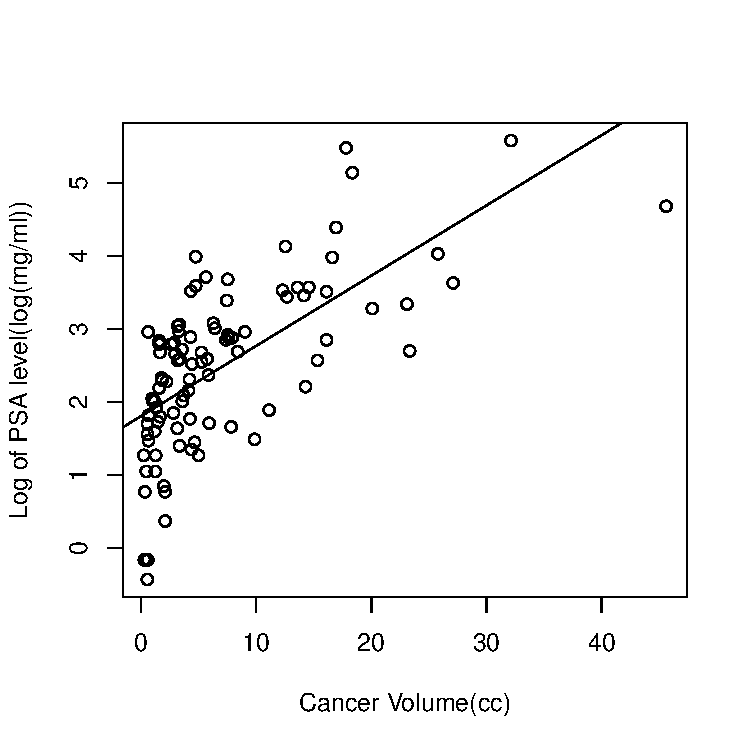
\includegraphics[width=.96\textwidth]{fig/boxplotcancervol.pdf}
    \end{subfigure}%
    ~
    \begin{subfigure}[t]{0.5\textwidth}
        \centering
        \caption{Weight ($weight$)}
        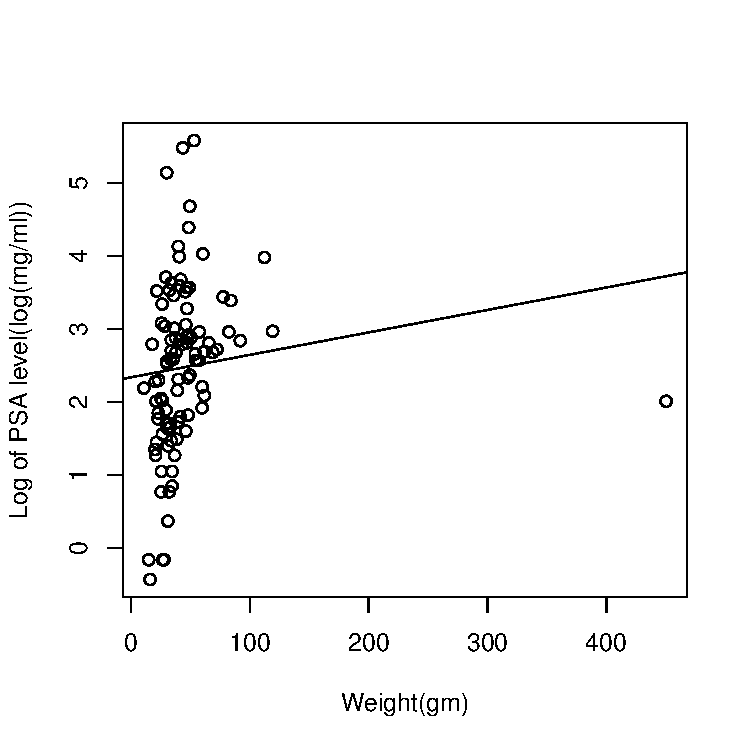
\includegraphics[width=.96\textwidth]{fig/boxplotweight.pdf}
    \end{subfigure}
    \\
    \begin{subfigure}[t]{0.5\textwidth}
        \centering
        \caption{Age ($age$)}
        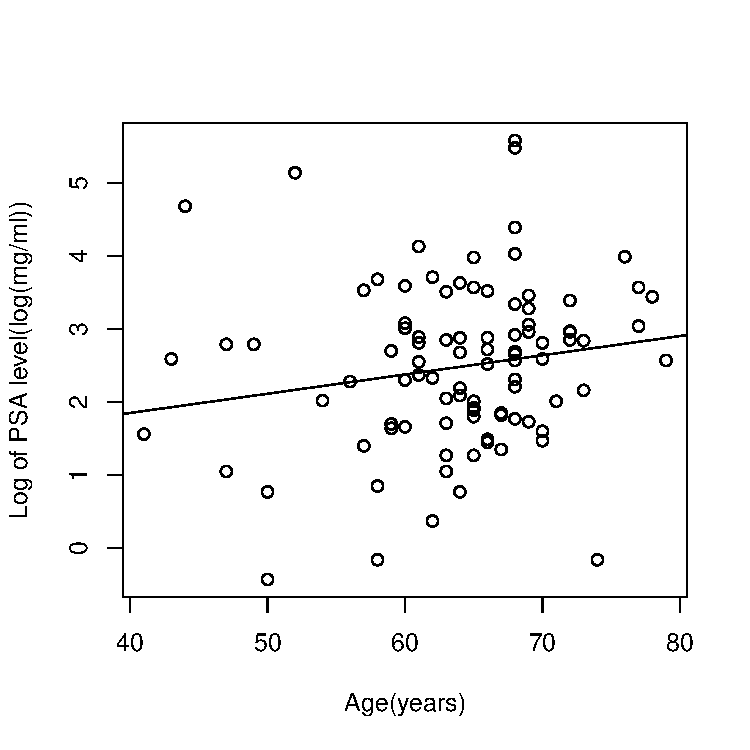
\includegraphics[width=.96\textwidth]{fig/boxplotage.pdf}
    \end{subfigure}%
    ~
    \begin{subfigure}[t]{0.5\textwidth}
        \centering
        \caption{Benign prostatic hyperplasia ($benpros$)}
        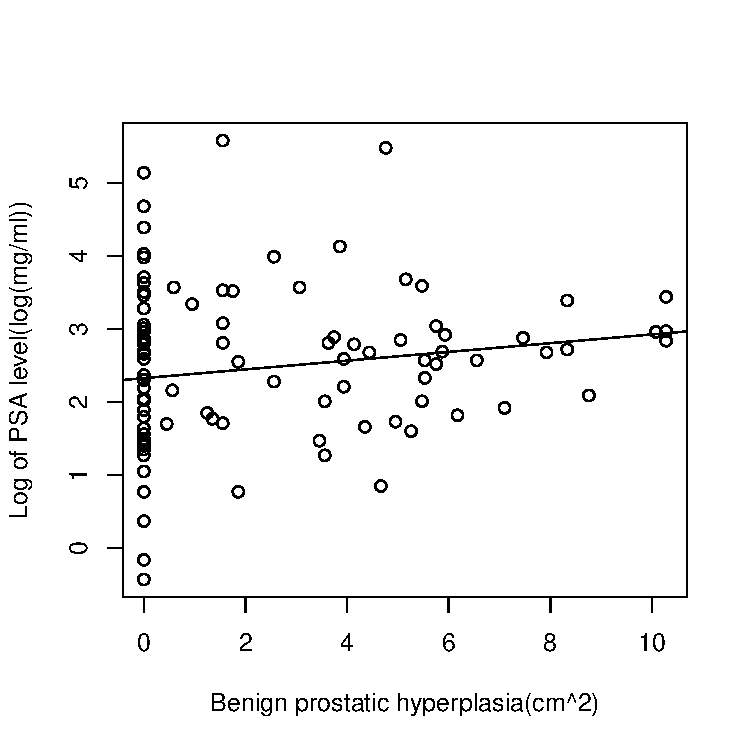
\includegraphics[width=.96\textwidth]{fig/boxplotbenpros.pdf}
    \end{subfigure}
    \\
    \begin{subfigure}[t]{0.5\textwidth}
        \centering
        \caption{Capsular penetration ($capspen$)}
        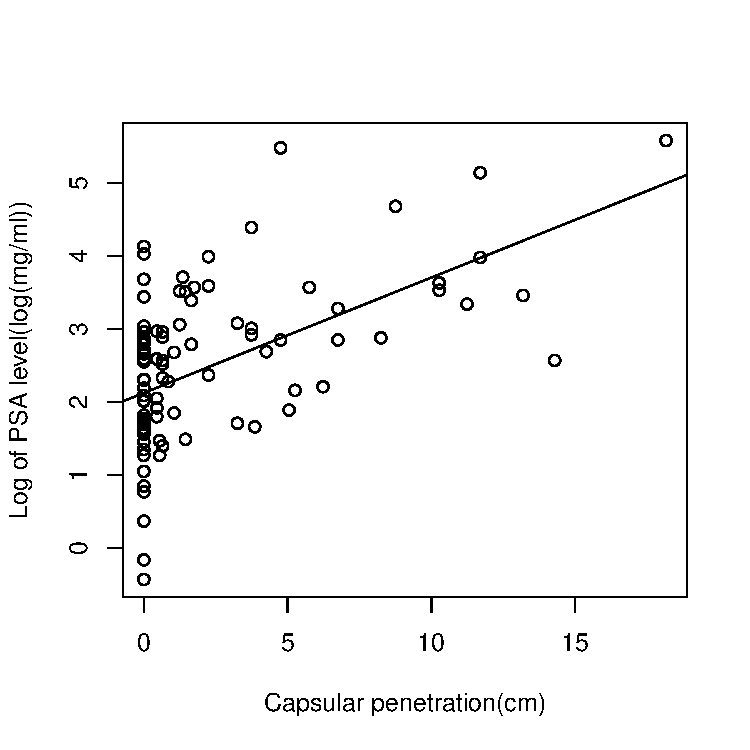
\includegraphics[width=.96\textwidth]{fig/boxplotcapspen.pdf}
    \end{subfigure}%
    \caption{Scatterplots for Different Variables}\label{b1}
\end{figure}


Based on these plots, we may have a guess that the most likely factors are 
\begin{enumerate}
\item Cancer Volume ($cancervol$)
\item Benign prostatic hyperplasia ($benpros$) 
\item Capsular penetration ($capspen$)
\end{enumerate}

Now we have two models, one containing three variables ($cancervol$, $benpros$and $capspen$), the other having all quantitative variables. And we compare these two models by doing an F test.



\begin{lstlisting}
> # Calculate the first formula.
> fit1 <- lm(psalog ~ cancervol + capspen + weight + age + benpros)
> fit1

Call:
lm(formula = psalog ~ cancervol + capspen + weight + age + benpros)

Coefficients:
(Intercept)    cancervol      capspen       weight          age      benpros
   1.037961     0.088925     0.033572     0.001028     0.007634     0.082325

> fit2 <- lm(psalog ~ cancervol + capspen + benpros)
> fit2

Call:
lm(formula = psalog ~ cancervol + capspen + benpros)

Coefficients:
(Intercept)    cancervol      capspen      benpros
    1.53504      0.08924      0.03544      0.09449

> # Compare first two guess.
> anova(fit2, fit1)
Analysis of Variance Table

Model 1: psalog ~ cancervol + capspen + benpros
Model 2: psalog ~ cancervol + capspen + weight + age + benpros
  Res.Df    RSS Df Sum of Sq      F Pr(>F)
1     93 63.904
2     91 63.430  2   0.47464 0.3405 0.7123
\end{lstlisting}

We can clearly see that:
\begin{enumerate}
\item $\beta_{weight}$ and $\beta_{age}$ are very small
\item $\beta_{cancervol}$, $\beta_{capspen}$ and $\beta_{benpros}$ are acceptably large
\item  $p$ value is also large ($0.7123$).
\end{enumerate}  Hence, we accept the null hypothesis that $\beta_{weight} = 0$ and $\beta_{age} = 0$.


Let us now conduct the stepwise selection to confirm our assumptions.

\begin{lstlisting}
> # Apply stepwise selection.
> # Forward selection based on AIC.
> fit3.forward <-
+     step(lm(psalog ~ 1),
+     scope = list(upper = ~ cancervol + capspen + weight + age + benpros),
+     direction = "forward")

> fit3.forward

Call:
lm(formula = psalog ~ cancervol + benpros)

Coefficients:
(Intercept)    cancervol      benpros
     1.5309       0.1010       0.0949

> # Backward elimination based on AIC.
> fit3.backward <-
+     step(lm(psalog ~ cancervol + capspen + weight + age + benpros),
+     scope = list(lower = ~1),
+     direction = "backward")

> fit3.backward

Call:
lm(formula = psalog ~ cancervol + benpros)

Coefficients:
(Intercept)    cancervol      benpros
     1.5309       0.1010       0.0949

>
> # Both forward/backward.
> fit3.both <-
+     step(lm(psalog ~ 1),
+     scope = list(lower = ~1,
+                  upper = ~ cancervol + capspen + weight + age + benpros),
+     direction = "both")

> fit3.both

Call:
lm(formula = psalog ~ cancervol + benpros)

Coefficients:
(Intercept)    cancervol      benpros
     1.5309       0.1010       0.0949
\end{lstlisting}

From the AIC value (which is omitted above) and recommended formula,
we now have a new formula:
\begin{lstlisting}
> # Model selected.
> fit3 <- lm(formula = psalog ~ cancervol + benpros)

> summary(fit3)

Call:
lm(formula = psalog ~ cancervol + benpros)

Residuals:
     Min       1Q   Median       3Q      Max
-2.01672 -0.55101  0.06457  0.56870  1.75415

Coefficients:
            Estimate Std. Error t value Pr(>|t|)
(Intercept)  1.53090    0.13940  10.982  < 2e-16 ***
cancervol    0.10105    0.01085   9.314 5.29e-15 ***
benpros      0.09490    0.02821   3.364  0.00111 **
---
Signif. codes:  0 '***' 0.001 '**' 0.01 '*' 0.05 '.' 0.1 ' ' 1

Residual standard error: 0.8303 on 94 degrees of freedom
Multiple R-squared:  0.4928,    Adjusted R-squared:  0.482
F-statistic: 45.67 on 2 and 94 DF,  p-value: 1.389e-14
\end{lstlisting}
We can compare it with our previous model having 3 quantitative predictors:
\begin{lstlisting}
> # Compare the model with the guess one.
> anova(fit3, fit2)
Analysis of Variance Table

Model 1: psalog ~ cancervol + benpros
Model 2: psalog ~ cancervol + capspen + benpros
  Res.Df    RSS Df Sum of Sq      F Pr(>F)
1     94 64.802
2     93 63.904  1   0.89737 1.3059 0.2561
\end{lstlisting}

The $p$ value is large ($0.2561$), and hence we accept the null hypothesis that $\beta_{capspen} = 0$. So we can now do away with variable $capspen$.


\pagebreak

The residual graph for the model using only quantitative variables is shown in \cref{rgmq}.
The absolute residual of the model is shown in \cref{abrgmq}.
\begin{figure}[H]
    \centering
    \begin{subfigure}[t]{0.5\textwidth}
        \centering
        \caption{Residual Graph}\label{rgmq}
        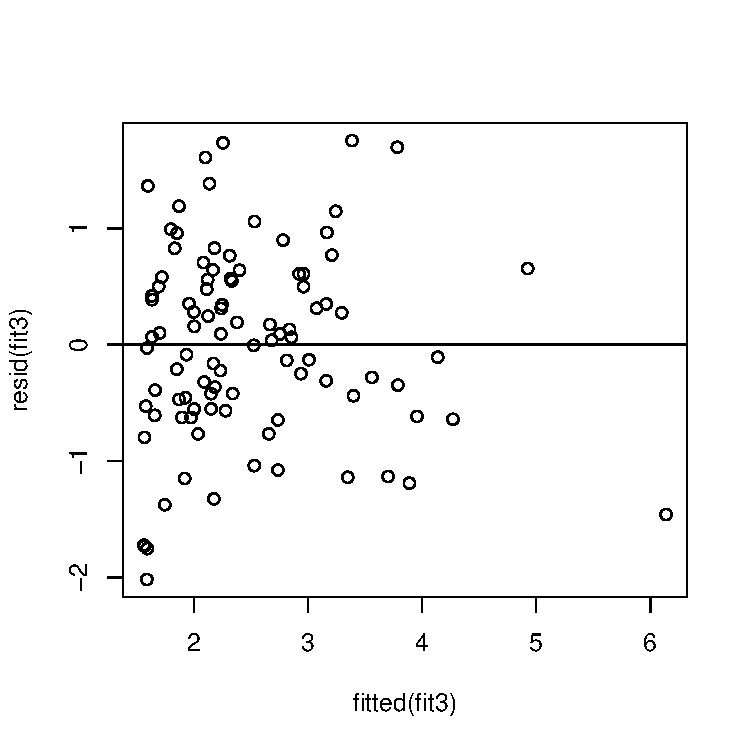
\includegraphics[width=.95\textwidth]{fig/residualplotfit3.pdf}
    \end{subfigure}%
    ~
    \begin{subfigure}[t]{0.5\textwidth}
        \centering
        \caption{Absolute Residual Graph}\label{abrgmq}
        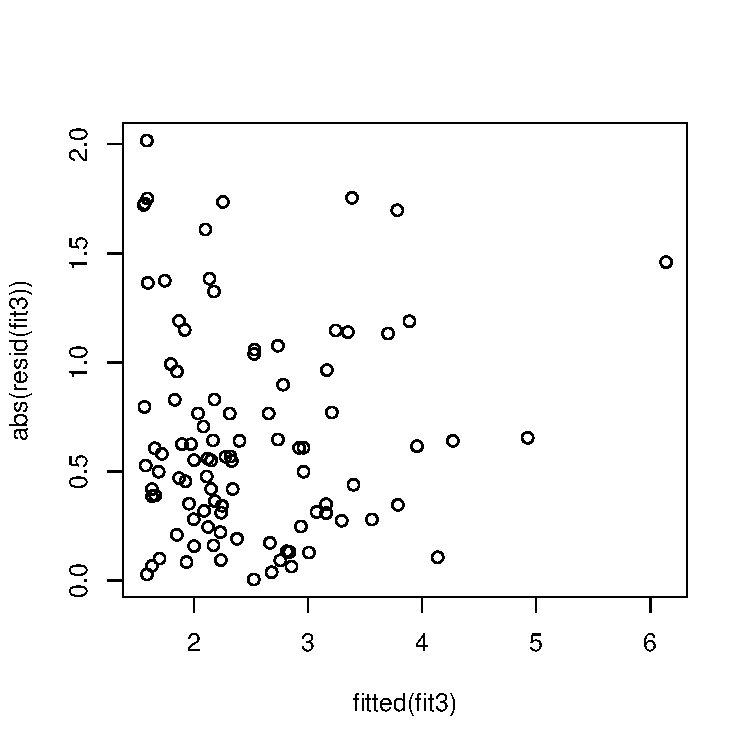
\includegraphics[width=.95\textwidth]{fig/plotfit3abu.pdf}
    \end{subfigure}
    \caption{Residual and Absolute Residual Graph for Model with only Quantitative Variables}
\end{figure}

The time series plot of the model is shown in \cref{timefit3}.
\begin{figure}[H]
    \centering
    \caption{Time Series Plot for the model with only quantitative variables}\label{timefit3}
    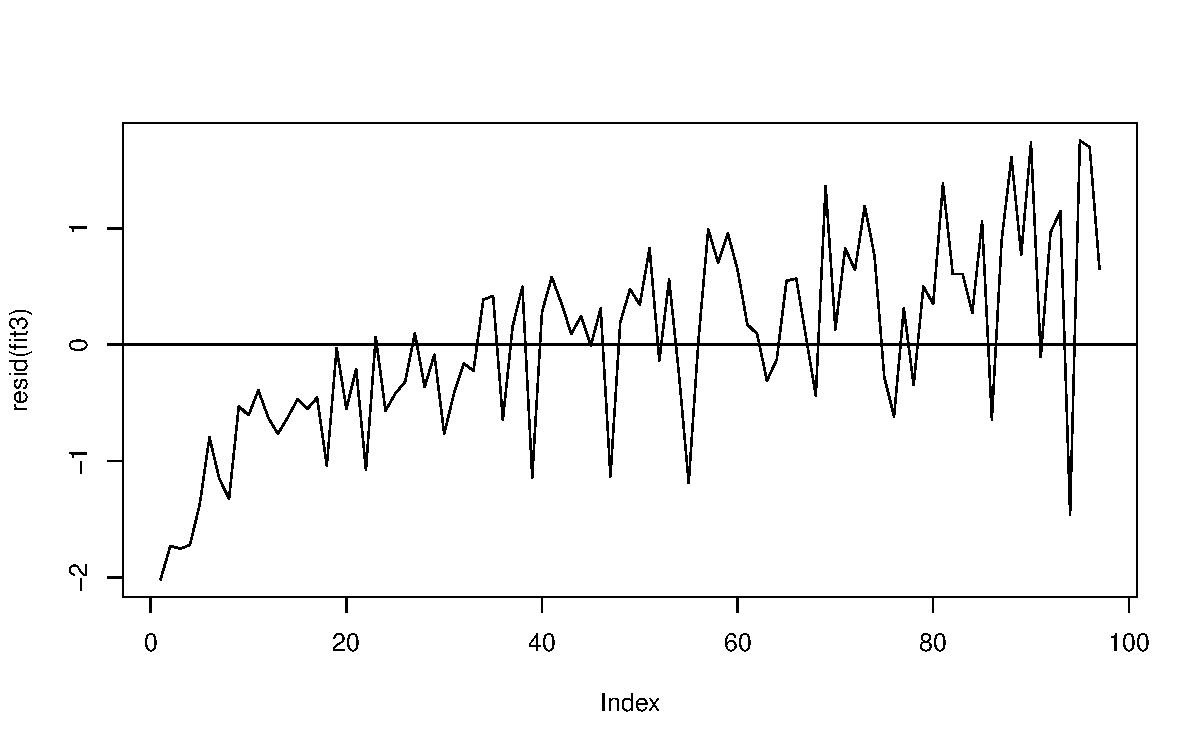
\includegraphics[width=.9\textwidth]{fig/plotfit3times.pdf}
\end{figure}

The normal QQ plot of the model is shown in \cref{qqfit3}.

\begin{figure}[H]
    \centering
    \caption{Normal QQ Plot for Model with Quantitative Variables Only}\label{qqfit3}
    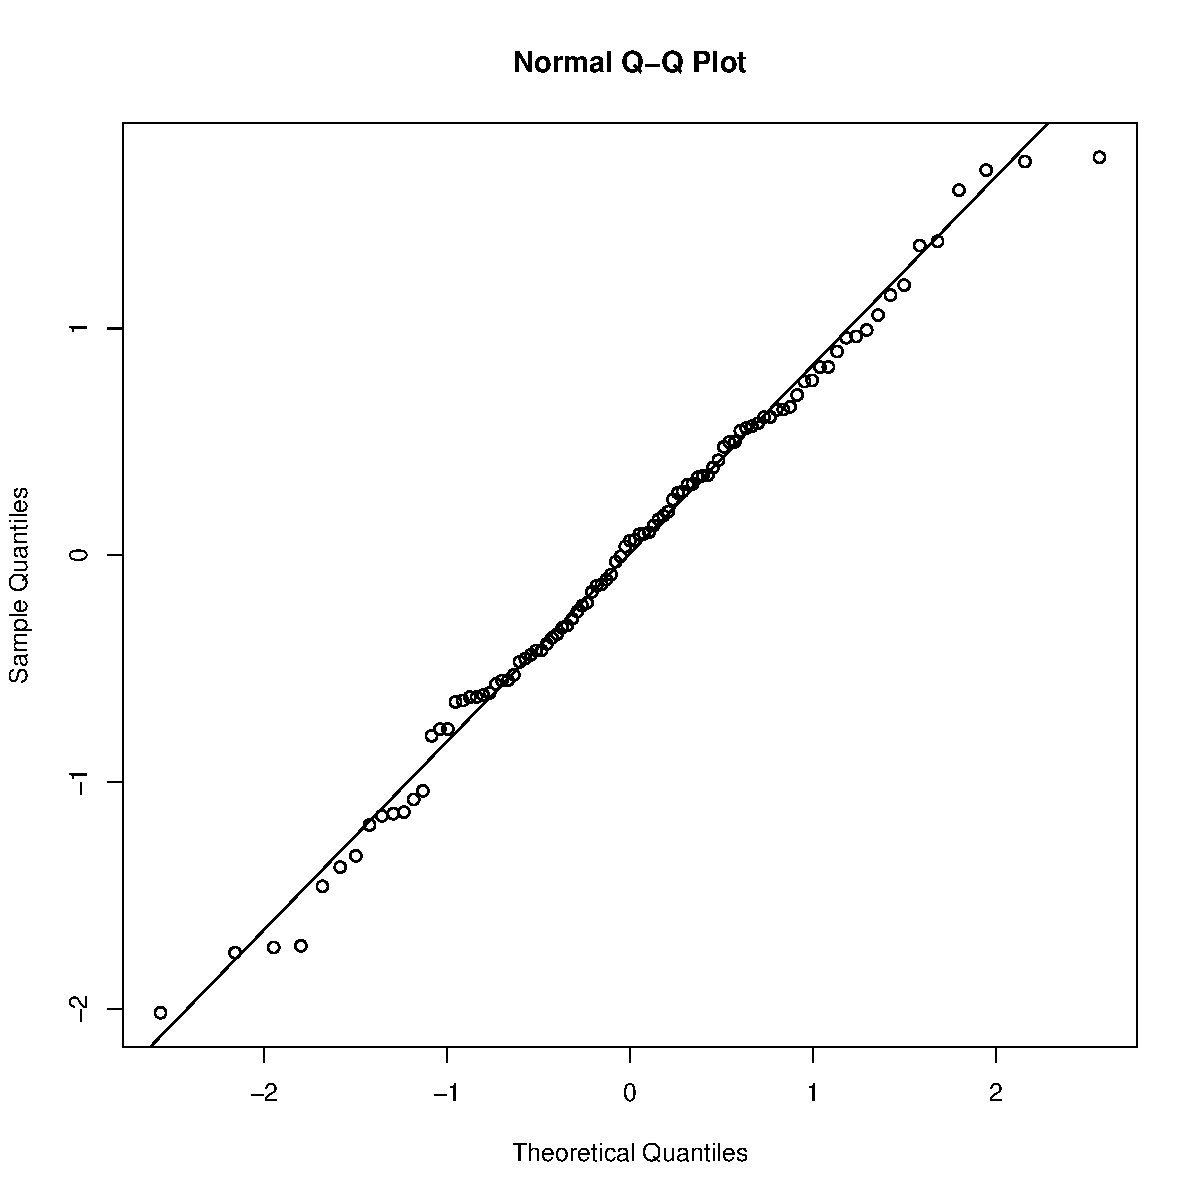
\includegraphics[width=.85\textwidth]{fig/qqnormplotfit3.pdf}
\end{figure}

The model seems quite reasonable. \\

We now proceed to consider the qualitative (categorical) variables. We first add two variables to the model separately and

\begin{lstlisting}
> # Consider the categorical variables.
> fit4 <- update(fit3, . ~ . + factor(vesinv))
> fit5 <- update(fit3, . ~ . + factor(gleason))
\end{lstlisting}

We compare these models (fit4 and fit5) with the fit3 model.
\begin{lstlisting}
> # Comparing two categorical variables.
> summary(fit5)

Call:
lm(formula = psalog ~ cancervol + benpros + factor(gleason))

Residuals:
     Min       1Q   Median       3Q      Max
-1.92886 -0.59159  0.04246  0.56555  1.56306

Coefficients:
                 Estimate Std. Error t value Pr(>|t|)
(Intercept)       1.34533    0.16164   8.323 7.63e-13 ***
cancervol         0.08095    0.01259   6.430 5.62e-09 ***
benpros           0.08622    0.02722   3.167  0.00209 **
factor(gleason)7  0.37475    0.18572   2.018  0.04652 *
factor(gleason)8  0.84137    0.26303   3.199  0.00189 **
---
Signif. codes:  0 '***' 0.001 '**' 0.01 '*' 0.05 '.' 0.1 ' ' 1

Residual standard error: 0.7942 on 92 degrees of freedom
Multiple R-squared:  0.5458,    Adjusted R-squared:  0.5261
F-statistic: 27.64 on 4 and 92 DF,  p-value: 4.467e-15

> anova(fit3, fit5)
Analysis of Variance Table

Model 1: psalog ~ cancervol + benpros
Model 2: psalog ~ cancervol + benpros + factor(gleason)
  Res.Df    RSS Df Sum of Sq      F   Pr(>F)
1     94 64.802
2     92 58.032  2    6.7695 5.3659 0.006249 **
---
Signif. codes:  0 '***' 0.001 '**' 0.01 '*' 0.05 '.' 0.1 ' ' 1

> summary(fit4)

Call:
lm(formula = psalog ~ cancervol + benpros + factor(vesinv))

Residuals:
    Min      1Q  Median      3Q     Max
-1.9867 -0.4996  0.1032  0.5545  1.4993

Coefficients:
                Estimate Std. Error t value Pr(>|t|)
(Intercept)      1.51484    0.13206  11.471  < 2e-16 ***
cancervol        0.07618    0.01256   6.067 2.78e-08 ***
benpros          0.09971    0.02674   3.729 0.000331 ***
factor(vesinv)1  0.82194    0.23858   3.445 0.000858 ***
---
Signif. codes:  0 '***' 0.001 '**' 0.01 '*' 0.05 '.' 0.1 ' ' 1

Residual standard error: 0.7861 on 93 degrees of freedom
Multiple R-squared:  0.5502,    Adjusted R-squared:  0.5357
F-statistic: 37.92 on 3 and 93 DF,  p-value: 4.247e-16

> anova(fit3, fit4)
Analysis of Variance Table

Model 1: psalog ~ cancervol + benpros
Model 2: psalog ~ cancervol + benpros + factor(vesinv)
  Res.Df    RSS Df Sum of Sq      F    Pr(>F)
1     94 64.802
2     93 57.468  1    7.3339 11.868 0.0008583 ***
---
Signif. codes:  0 '***' 0.001 '**' 0.01 '*' 0.05 '.' 0.1 ' ' 1
\end{lstlisting}

We see that both these variables \textit{vesinv} and \textit{gleason} are definitely
significant to the model.\\
 So we add these two variables to the formula, which results in our final model.
\begin{lstlisting}
> # Finalize the model.
> fit6 <- update(fit3, . ~ . + factor(vesinv) + factor(gleason))
>
> summary(fit6)

Call:
lm(formula = psalog ~ cancervol + benpros + factor(vesinv) +
    factor(gleason))

Residuals:
     Min       1Q   Median       3Q      Max
-1.85235 -0.45777  0.06741  0.51651  1.53204

Coefficients:
                 Estimate Std. Error t value Pr(>|t|)
(Intercept)       1.38817    0.15609   8.894 5.27e-14 ***
cancervol         0.06241    0.01367   4.566 1.55e-05 ***
benpros           0.09265    0.02627   3.527  0.00066 ***
factor(vesinv)1   0.69646    0.23837   2.922  0.00439 **
factor(gleason)7  0.26028    0.18280   1.424  0.15790
factor(gleason)8  0.70545    0.25712   2.744  0.00732 **
---
Signif. codes:  0 '***' 0.001 '**' 0.01 '*' 0.05 '.' 0.1 ' ' 1

Residual standard error: 0.7636 on 91 degrees of freedom
Multiple R-squared:  0.5848,    Adjusted R-squared:  0.5619
F-statistic: 25.63 on 5 and 91 DF,  p-value: 4.722e-16
\end{lstlisting}

\pagebreak
The residual graph for the final model is shown in \cref{rgmqf}.
The absolute residual of the model is shown in \cref{abrgmqf}.

\begin{figure}[H]
    \centering
    \begin{subfigure}[t]{0.5\textwidth}
        \centering
        \caption{Residual Graph}\label{rgmqf}
        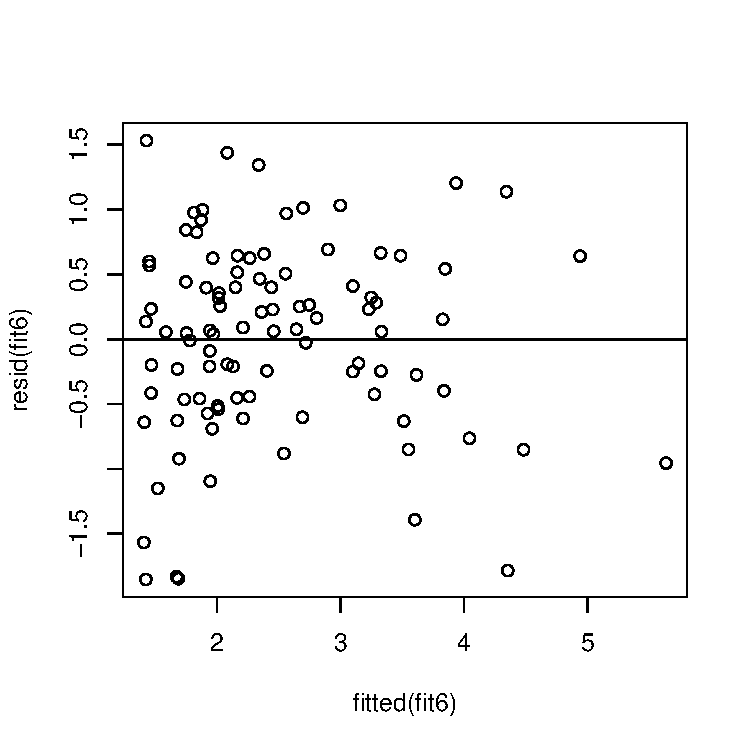
\includegraphics[width=.95\textwidth]{fig/residualplotfit6.pdf}
    \end{subfigure}%
    ~
    \begin{subfigure}[t]{0.5\textwidth}
        \centering
        \caption{Absolute Residual Graph}\label{abrgmqf}
        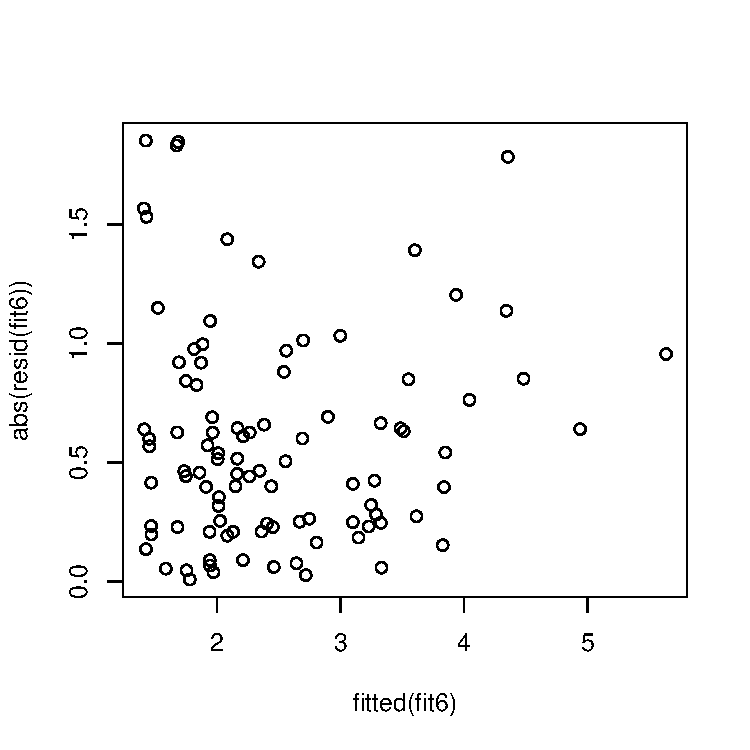
\includegraphics[width=.95\textwidth]{fig/plotfit6abu.pdf}
    \end{subfigure}
    \caption{Residual and Absolute Residual Graph for Final Model}
\end{figure}

The time series plot of the model is shown in \cref{timefit6}.
\begin{figure}[H]
    \centering
    \caption{Time Series Plot for Final Model}\label{timefit6}

    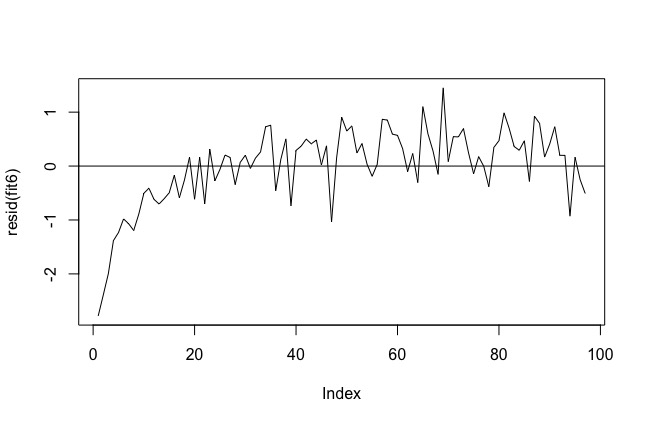
\includegraphics[width=.85\textwidth]{fig/fit6time.jpeg}

\end{figure}

The normal QQ plot of the model is shown in \cref{qqfit6}.

\begin{figure}[H]
    \centering
    \caption{Normal QQ Plot for Final Model}\label{qqfit6}
    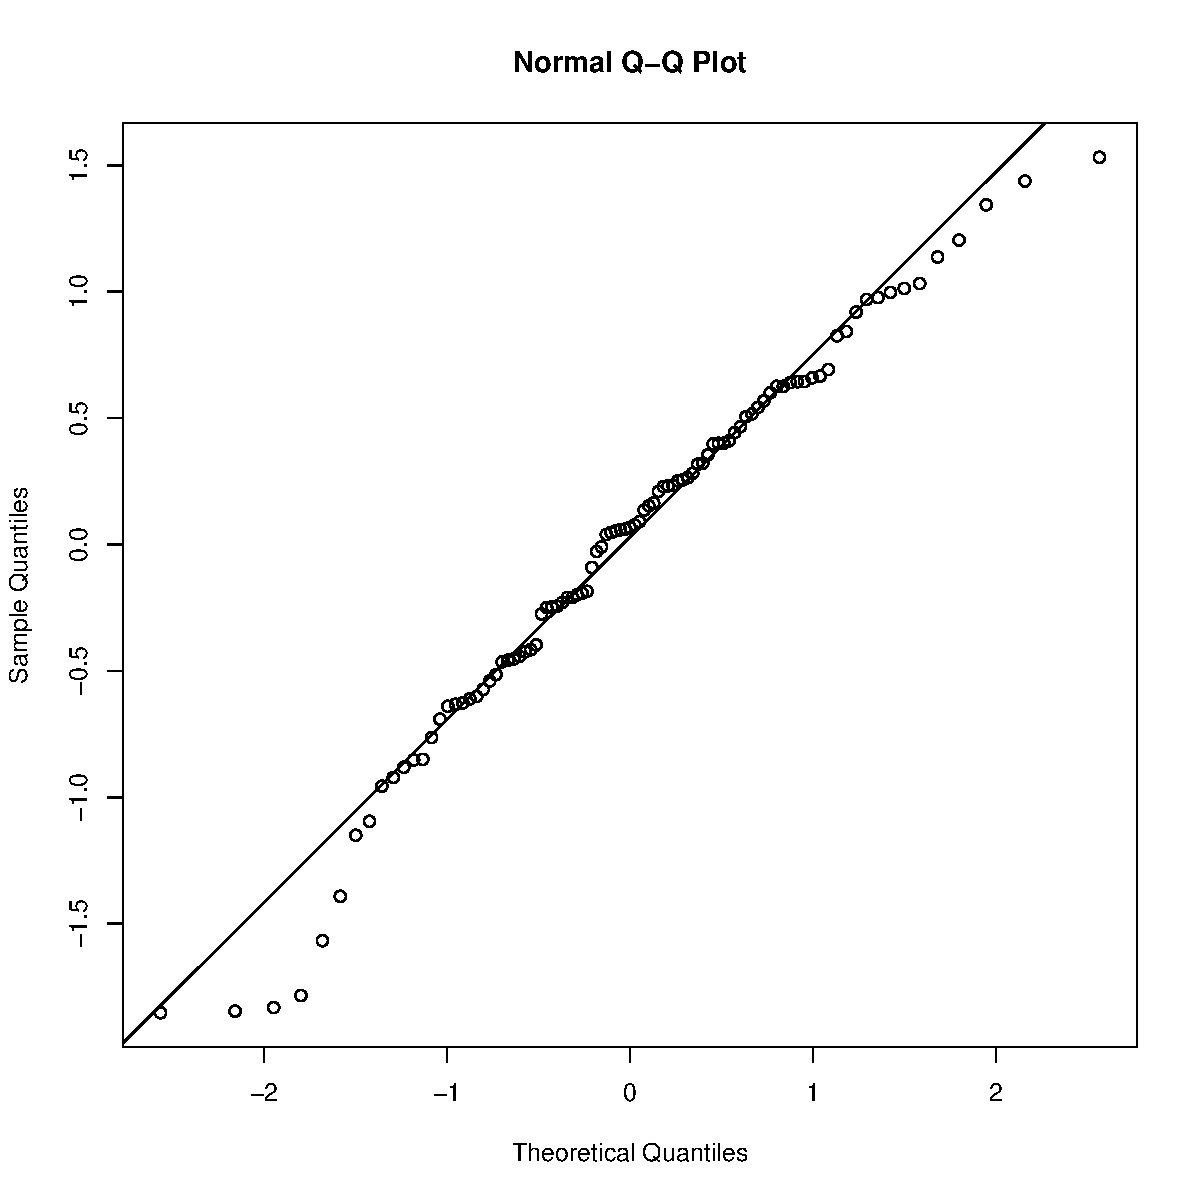
\includegraphics[width=.85\textwidth]{fig/qqnormplotfit6.pdf}
\end{figure}

The model seems reasonable in most part but has some outliers.

With this model we can now predict the PSA level for a patient whose quantitative predictors are at their sample means and qualitative predictors are at their sample modes.
\begin{lstlisting}
> # Predict the PSA level for sample mean.
> pred <- predict(fit6,
+     data.frame(cancervol = mean(cancervol),
+                benpros   = mean(benpros),
+                vesinv    = getmode(vesinv),
+                gleason   = getmode(gleason)))
> exp(pred)
       1
10.17628
\end{lstlisting}

\pagebreak

\section{R Code}
\lstinputlisting{/users/psprao/downloads/stats/mini6/mini_project5.R}

\end{document}
